\documentclass[output=paper]{LSP/langsci}  
\author{Anne-Sophie Ghyselen\affiliation{Ghent University}} 
\title{From diglossia to diaglossia: {A} {W}est {F}lemish case-study}
  
\abstract{
\citet{auer_europes_2005,auer_dialect_2011} distinguishes five types of dialect/standard constellations in Europe, which stand in a diachronic relationship and of which the diaglossic repertoire, marked by intermediate forms between standard and dialect, would be the most widespread in Europe today. While a lot of current research focuses on contemporary shifts in diaglossic situations towards dialect loss (cf. \citealt{vandekerckhove_dialect_2009}), shifts from diglossia to diaglossia remain relatively understudied (cf. \citealt[23]{auer_europes_2005}). The present paper reports on the West \il{Dutch!Flemish}Flemish area, where the language is said to be evolving from a diglossic to a diaglossic situation (\citealt{de_caluwe_tussentaal_2009}, \citealt[272]{willemyns_-standardization_2007}). In order to tap into the structure of this West \il{Dutch!Flemish}Flemish repertoire, the language use of 10 speakers from Ypres is analysed systematically by means of a correspondence analysis of 26 phonological and morphosyntactic variables in five speech settings. These analyses show that in West Flanders, the emerging intermediate variations are mainly used in supraregional informal settings, illustrating the need to focus on this at present understudied speech setting when studying changing repertoires. The data clearly indicate that in the incipient transition from diglossia to diaglossia, both dialect and (an intended form of) standard language are still vital as means of regional informal and supraregional formal communication respectively. Structurally, the intermediate variations mainly result from dialect-to-standard convergence, but some speakers also show horizontal dialect convergence.
}

\maketitle 
\begin{document}

\newcommand{\ghysvara}{[-st,+ypr]~}
\newcommand{\ghysvarb}{[+st,+ypr]~}
\newcommand{\ghysvarc}{[-st,-ypr]~}
\newcommand{\ghysvard}{[+st,-ypr]~}
%%% We could even add colour back in, as long as the symbols/variables are ALSO clear without colour
%%%%SN: correct
%%% OS: I've added back colours to further emphasise the variable differences so people can see them quickly; removed the superscript on the variables, because they popped just outside of the coloured cell areas. We could also make it text colour instead of cell colour, if that looks better.

%versions WITH color:
%\newcommand{\ghysvara}{\cellcolor{red!36}[-st,+ypr]~}
%\newcommand{\ghysvarb}{\cellcolor{red!18}[+st,+ypr]~}
%\newcommand{\ghysvarc}{\cellcolor{blue!36}[-st,-ypr]~}
%\newcommand{\ghysvard}{\cellcolor{blue!18}[+st,-ypr]~}

\newcommand{\tabitem}{{\textbullet}~~}
 
 

\section{Introduction}
\label{sec:introduction}

All over Europe factors such as geographical and social mobility, a high level of education, the growing impact of mass media and a general decreasing level of formality in public life have caused various types of language change \citep[355]{taeldeman_linguistic_2009}. \citet{heeringa_convergence_2014} for instance find convergence between dialect varieties and dialect groups in the \ili{Dutch} language area, \citet{cheshire_contact_2011} report on the emergence of Multicultural London English, \citet{auer_demotisation_2011} find homogenisation of the spoken standard across Germany, and according to \citet{kristiansen_two_2001} a double standard norm is emerging in Denmark. These are only some examples of the many studies reporting contemporary language change in Europe. The described changes at first sight appear very diverse and language-specific, but as \citet[7]{auer_europes_2005} argues, “on a sufficient level of generalization there is a systematicity behind the superficial heterogeneity”. He distinguishes five types of dialect/standard constellations, which stand in a diachronic relationship and of which the diaglossic repertoire, marked by intermediate forms between standard and dialect, would be the most widespread in Europe today. While a lot of current research focuses on contemporary shifts in diaglossic situations towards \isi{dialect loss} (cf. \citealt{ghyselen_impact_2013,grondelaers_standard_2011,vandekerckhove_dialect_2009}), “the exact nature of the transition from diglossia to diaglossia is not yet clear” \citep[23]{auer_europes_2005}. Which pragmatic functions are initially allocated to the newly emerged intermediate variations? To what degree does the change from \isi{diglossia} to \isi{diaglossia} imply dialect loss, either structural or functional \citep{auer_convergence_1996}? What impact do the new intermediate variations have on the structure and function of the standard language? How do new intermediate variations structurally take shape? To gain insight into these issues, the present paper reports on the West \il{Dutch!Flemish}Flemish dialect area, where the repertoire is said to be evolving from a diglossic one into a diaglossic one (\citealt{de_caluwe_tussentaal_2009}, \citealt[272]{willemyns_-standardization_2007}). To tap into the structure of this West \il{Dutch!Flemish}Flemish repertoire and the functionality of its components, the language use of 10 speakers from Ypres is analysed systematically. A correspondence analysis of 26 phonological and morphosyntactic variables in five speech settings shows that in Ypres, some speakers still have diglossic repertoires, whereas others have diaglossic ones. The latter speakers use intermediate variations in supraregional informal settings, but speak dialect and standard language in informal regional and formal supraregional settings respectively. This variation between repertoire structures indicates that in the West \il{Dutch!Flemish}Flemish incipient transition from diglossia to diaglossia, both dialect and (an intended form of) standard language are still vital as means of respectively regional informal and supraregional formal communication. Structurally, the intermediate variations mainly result from dialect-to-standard convergence; some speakers however also show horizontal dialect convergence.

\section{Language variation and change in Flanders}
\label{sec:Flanders}

In this study, the term \textit{Flanders} is used in its political sense to refer to the northern, \ili{Dutch} speaking part of Belgium.\footnote{In its dialectological sense, the notion \textit{Flanders} refers to the area where the West, East, French, and Zeeuws \il{Dutch!Flemish}Flemish dialects are spoken. This area coincides with the old county of Flanders and comprises the western part of northern Belgium, northern France, and the southwest of the Netherlands.} This area shares a standard language with the Netherlands, although it has developed its own national variety, i.e. Belgian \ili{Dutch} (cf. \citealt{grondelaers_standard_2011}). The Belgian \ili{Dutch} standard language is in its spoken form often referred to as ‘VRT-\ili{Dutch}’, as it is the variety used by official broadcasters on the Vlaamse Radio- en Televisieomroep (VRT), the \il{Dutch!Flemish}Flemish public broadcaster. This VRT-\ili{Dutch} is often said to be a mainly virtual colloquial variety, as it is desired by the authorities, but rarely spoken in practice \citep[19]{de_caluwe_tussentaal_2009}. Instead, in daily life, non-standard language is ubiquitous. A wide variety of dialects can for instance be heard when travelling through Flanders. These dialects are traditionally classified into four main dialect groups (cf. figure {fig:ghys:Flanders}): the West \il{Dutch!Flemish}Flemish, East-\il{Dutch!Flemish}Flemish, Brabantic and Limburgian dialects (cf. \citealt{vandekerckhove_dialect_2009}). Moreover, intermediate language use between dialect and standard language (the so-called \textit{"tussentaal"}\is{tussentaal}\footnote{See \citet{ghyselen_stabilisering_forthcoming} on the way in which dialect can be distinguished from \textit{tussentaal.}}) is increasingly prevalent \citep{de_caluwe_tussentaal_2006}, turning the \il{Dutch!Flemish}Flemish language repertoire into a largely diaglossic repertoire (cf. \sectref{sec:ditodia}).

\begin{figure}
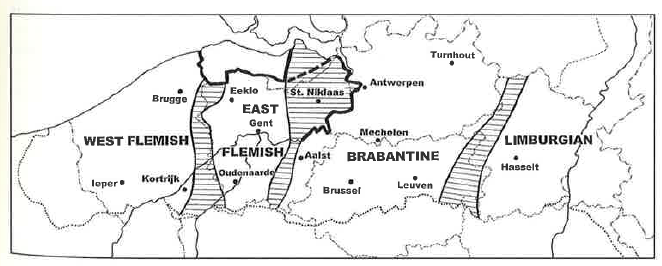
\includegraphics[width=\textwidth]{illustrations/ghys_fig1.png}
\caption{Dialect areas in Flanders; based on \citet[359]{taeldeman_linguistic_2009}.}
\label{fig:ghys:Flanders}
\end{figure}

\largerpage
Since the Nineties, the status of both dialects and standard language in Flanders has changed significantly, just as in many other European language communities. Dialect studies have shown that the dialects in Flanders are suffering from both functional \citep{ghyselen_dialectcompetentie_2014} and structural \citep{heeringa_convergence_2014,vandekerckhove_structurele_2000} loss:\footnote{See \citet{ghyselen_dialectcompetentie_2014} for an in-depth discussion of the distinction between functional and structural dialect loss.} increasingly fewer people are speaking dialect in increasingly fewer situations, and those who still speak their local dialect are using fewer and fewer local dialect features. In this process of dialect loss clear regional differences can be distinguished: whereas dialect loss has progressed furthest in East Flanders, Brabant and Limburg, West Flanders (and especially the south-western part of this area) still shows considerable dialect vitality (cf. \citealt{ghyselen_dialectcompetentie_2014}). The observed functional dialect loss mainly benefits the use of intermediate language \citep{de_caluwe_tussentaal_2006}, although \textit{tussentaal} does not seem to be the mere result of dialect loss. \textit{Tussentaal} would also function as a ‘lingua franca’ in informal settings where dialect speakers from different areas meet (cf. \citealt{gabel_taalaccommodatie_2010}). 

At the standard end of the language repertoire, several processes of language change have been observed as well. \citet{plevoets_tussen_2008} concludes on the basis of an extensive corpus study that speakers born in the 50s and 60s of the previous century frequently use Standard \ili{Dutch}, whereas those from the 70s and 80s are more prone to speak \textit{tussentaal}. \citet{delarue_teachers_2013} observes in the same vein that several teachers aged 50 or older speak exclusively Standard \ili{Dutch} in their classes, whereas younger teachers tend to use non-standard variants more frequently while teaching. These observations point towards ``standard loss'' in Flanders, although it has to be borne in mind that this loss pertains mainly to the spoken standard: as \citet[9]{grondelaers_standard_2011b} and \citet{vandekerckhove_belgian_2005} emphasise, the written standard in Flanders is fairly resistant to change. While increasing numbers of empirical studies focus on the changing position of the standard language in Flanders (see e.g. \citealt{plevoets_tussen_2008}), a number of issues continue to be highly controversial. One of these is the shape of the change process, namely whether the ``standard loss'' in Flanders should be thought of as an instance of \isi{destandardisation} “whereby the established standard language loses its position as the one and only ‘best language’” \citep[28]{coupland_slice:_2011}, or rather as \isi{demotisation}, i.e. the process whereby the “‘standard ideology’ as such stays intact while the valorisation of ways of speaking changes” \citep[28]{coupland_slice:_2011}. Related to this question is the debate on the potential ‘stabilisation of \textit{tussentaal}’, that is whether one more or less homogeneous \textit{tussentaal} is emerging, as suggested in \citet{willemyns_verkavelingsbrabants._2005} for instance. For a discussion of the relationship between the homogeneisation of \textit{tussentaal} on the one hand and demotisation and destandardisation on the other, see \citet{ghyselen_stabilisering_forthcoming}.

\section{From diglossic to diaglossic repertoires}
\label{sec:ditodia}

\citet{auer_europes_2005,auer_dialect_2011} distinguishes five macrotypes of dialect/standard constellations. The first two types, the exoglossic diglossia and the medial diglossia, will not be elaborated on here, as these are rare in Europe and do not occur in Flanders. The types which are of interest in this chapter, are the third, fourth and fifth repertoire types, respectively the spoken diglossia, the diaglossic repertoire, and the dialect loss repertoire. Spoken diglossia are generally defined as repertoires in which the spoken standard is strictly separated, both structurally and functionally, from the local dialects. These varieties each have specific pragmatic functions, which force speakers to code-switch depending on the situation they are in. The diaglossic repertoire, however, is marked by intermediate variants between standard and dialect. In this repertoire type, there are not only code-switches between dialect and the standard, but speakers can also make subtler shifts from a more dialectal variant to a more standard one. These shifts have been accounted for in relation to the attention a speaker devotes to his or her speech \citep[208]{labov_sociolinguistic_1972} and to several situational parameters, such as the (language use of) the speech partners \citep{bell_language_1984}, the conversational topic or the medium \citep{giles_speech_1975}. Recent approaches to \isi{style-shifting}, however, argue that style shifts are not merely triggered by external parameters, but that speakers can also actively use them to construct social meaning and to act out identities which may for instance not be symbolised through the base dialect (\citealt[23]{auer_europes_2005}, \citealt[378]{schilling-estes_investigating_2002}). The precise mechanisms by which diaglossia evolve out of diglossia are at present not clear and many questions remain. For example, what pragmatic functions are initially allocated to the newly emerging intermediate variations in diaglossic repertoires? What is the impact on the functionality of both dialect and standard language? From a more structural perspective, how do the intermediate variations take shape? \citet[25]{auer_europes_2005} suggests dialect change targeted towards the standard language as one of the main driving forces in the emergence of intermediate variations, but also highlights that this process may co-occur with destandardisation, implying that regional features are increasingly tolerated in the standard variety. In dialect loss situations, the fifth repertoire type discussed by \citet{auer_europes_2005,auer_dialect_2011}, destandardisation would occur even more frequently. It appears that the disappearance of the linguistic forms with the most restricted geographical reach stimulates processes of divergence from the national standard \citep[30]{auer_europes_2005}. According to \citet[30]{auer_europes_2005}, this divergence is steered by speakers’ “need to sound different from the codified standard”. 

Auer’s distinction between diglossia and diaglossia seems quite straightforward. However, in empirical studies, different approaches towards these concepts can be distinguished. \citet{rys_fonologische_2007} for instance label the \il{Dutch!Flemish}Flemish language repertoire as diaglossic because production data from Flanders show frequent non-dialectal, non-standard language. \citet{willemyns_diglossie_2008}, however, seem to take speaker intention as a central criterion: though they recognise that in West Flanders intermediate language use can be heard, they nonetheless argue that the repertoire in the western peripheral region is of a diglossic nature, as speakers would intend to speak either dialect or standard and perceive the language repertoire in a bipolar way. This distinction between production- and perception-oriented approaches is closely intertwined with a distinction between studies at the level of the individual speaker and those at the level of the speech community. Repertoire studies at these different levels can yield very different results; where individual speakers may have diglossic repertoires with a clear structural distance between dialect and some form of intended standard, a combination of all those individual repertoires may yield a diaglossic overall picture. In this study, I adopt a production-oriented approach focusing on the language use of individual speakers. If speakers code-switch between two structurally and functionally separate systems, their repertoire is labelled diglossic; if they dispose of more than two types of language use and make more subtle style-shifts, their repertoire is classified as diaglossic. On the level of the speech community, the shift from a diglossic to a diaglossic repertoire can therefore be characterised as a shift from a community in which most speakers show a diglossic individual repertoire to one in which most speakers have diaglossic individual repertoires. 

While the \il{Dutch!Flemish}Flemish language area is generally said to be diaglossic and evolving towards dialect loss, the language repertoire in West Flanders is still usually classed as largely diglossic (\citealt{de_caluwe_tussentaal_2009}, \citealt{willemyns_diglossie_2008}), with individual speakers making clear code-switches between dialect and some form of standard language. Recently, however, \citet{gabel_taalaccommodatie_2010} found that West \il{Dutch!Flemish}Flemish adolescents have more than two codes at their disposal; her study shows how adolescents switch to non-standard, non-dialectal language use in supraregional informal settings. This observation points towards changing repertoire structures in West Flanders, but as the supraregional informal language use of older speakers has not been studied so far – supraregional informal language as such has remained largely out of the picture in most variationist research – straightforward conclusions concerning ongoing changes are difficult to draw.

\section{Methodology}
\label{sec:methodology}

\largerpage
In order to study the potentially changing repertoires in West Flanders, this research analyses the linguistic repertoires of ten highly educated women\footnote{They all have a university degree, but they do not practice a language-oriented profession (no linguists, interpreters, journalists, speech therapists, actors or teachers).} from Ypres systematically by studying their language in several speech settings. This practice has a considerable tradition in German dialectology and variationist linguistics (cf. \citealt{kehrein_regionalsprachliche_2012}, \citealt{lenz_struktur_2003}, \citealt{stellmacher_studien_1977}) but is fairly novel in \ili{Dutch} sociolinguistics. The studied women were born between 1981 and 1986 (n=5) or between 1955 and 1961 (n=5)\footnote{ Speakers from the younger age group have the letter ‘a’ in the speaker code (e.g. wvla1), whereas the older speakers have the letter ‘b’ (e.g. wvlb1). I compared the language use of younger and older women, not of younger women and older men (contrary to \citealt{heeringa_convergence_2014}), as I did not want age effects to be confounded by gender effects. }, and were recorded in five speech settings: (1) a dialect test, (2) a standard language test, (3) a conversation with a friend\footnote{Gender was not controlled for in these conversations, as it was already difficult finding suitable informants without making demands on the gender of the speech partners. 6 of the 20 conversations with friends (of the same or of a different dialect area) were mixed-sex conversations, so the majority were same-sex conversations. This potentially confounding factor will be taken into account when discussing the results.} from the same city, (4) a conversation with a friend from a different dialect area and (5) a sociolinguistic interview with an unknown interviewer from a different dialect area. During the sociolinguistic interviews, data were gathered about the linguistic background of the informants and their perceptions of their own language use. In the dialect and standard tests, the informants heard stimuli sentences spoken in either standard \ili{Dutch} or in the local dialect, which they had to translate into respectively the dialect of the oldest people of their town and standard \ili{Dutch}  ``as heard during news broadcasts''. These tests were used to determine the informant’s proficiency in the most acrolectal versus basilectal speech styles available in a relevant location.\footnote{ The data obtained in the test settings are of a very different nature than the spontaneous speech data (cf. \citealt[57--62]{lenz_struktur_2003}). This difference will be taken into account when analyzing the results.} The gathered recordings were transcribed orthographically using Praat \citep{boersma_praat:_2011}\footnote{Of each conversation with a friend 30 minutes were transcribed; the interviews and dialect and standard tests were transcribed entirely.} and a searchable corpus was built using the software package EXMARaLDA \citep{schmidt_exmaralda_2009}.

The built corpus was analysed using a correlative sociolinguistic approach: the distributions of 26 phonological and morphosyntactic features were studied in the five types of data. In total, 22495 tokens were auditorily categorised into 60 variant categories by one linguist. To judge the objectiveness of these categorisations, a random sample of about 190 tokens was taken for each phonological variable, which was subsequently rated by a second linguist. If the inter-rater agreement proved to be too low (Cohen's kappa {\textless}0.61, cf. \citealt[165]{landis_measurement_1977}), the variable was excluded from the study. A list of the selected variables and their attested variants is given in Tables~\ref{tab:ghys:1a} and \ref{tab:ghys:1c}, where information is also given on the frequency of the variants and the variant type:\footnote{In order to make this distinction, benchmarks for both the standard and dialect were necessary. As benchmark for standardness, the pronunciation dictionary of \citet{heemskerk_uitspraakwoordenboek_2000} and the \textit{Algemeen Nederlandse Spraakkunst} \citep{ANS} were used. The Ypres dialect norm was determined using SAND (\citealt{barbiers_syntactische_2005}, \citealt{barbiers_syntactische_2008}), 
FAND (\citealt{de_wulf_fonologische_2005}, \citealt{goossens_fonologische_2000}, \citealt{goossens_fonologische_1998}) and 
MAND (\citealt{de_schutter_morfologische_2005}, \citealt{goeman_mand_2008}). For a number of variables, specialised dialectological descriptions were consulted (\citealt{cornips_variatie_2009} on gender in \ili{Dutch}, \citealt{de_vogelaer_nederlandse_2008} on subject marking, \citealt{de_vogelaer_iemand_2006} on indefinite pronouns and adverbs).}

\begin{enumerate}
\item {[-st,+ypr]}-variants, i.e. non-standard  variants endogenous in the dialect of Ypres;
\item {[+st,+ypr]}-variants, i.e. standard variants which also occur in the dialect of Ypres
\item {[-st,-ypr]}-variants, i.e. variants which do not occur in the standard, nor in the dialect of Ypres. 
\item {[+st,-ypr]}-variants, i.e. standard variants which do not occur in the dialect of Ypres;
\end{enumerate}
%%%
%%% check table references
%%%
The second column of \tabref{tab:ghys:1a} gives information on the regional spread of the [-st, +iep]-variants: (a) a region smaller than West Flanders, (b) West Flanders, (c) West and East Flanders or (d) an area larger than West and East Flanders. A last category of variables (category e) contains variables of which the [-ypr, -st]-variant occurs in almost all dialects in Flanders, except in the Ypres area. This information on the regional spread of the [-st] variants is highly relevant, as the regional spread of dialect features is known to strongly influence the dynamics of those features (cf. Schirmunski 1930, Taeldeman 2009). Since it would involve going too far afield to discuss all of the 23 variables in detail, I refer to 
SAND (\citealt{barbiers_syntactische_2005}, \citealt{barbiers_syntactische_2008}), 
FAND (\citealt{de_wulf_fonologische_2005}, \citealt{goossens_fonologische_2000}, \citealt{goossens_fonologische_1998}), 
MAND (\citealt{de_schutter_morfologische_2005}, \citealt{goeman_mand_2008}), \citet{de_vogelaer_nederlandse_2008}, \citet{cornips_variatie_2009} and \citet{de_vogelaer_iemand_2006} for detailed information. \citet{ghyselen_stabilisering_forthcoming} describes how the variables were selected. 

To study how the attested variants correlate to each other and to the independent variables (age and speech setting), profile-based Multiple Correspondence Analysis was performed (cf. \citealt{de_sutter_lexical_2012}, \citealt{plevoets_tussen_2008}) with age, speech setting and speaker as independent variables. Multiple Correspondence Analysis (MCA) is a descriptive data analysis technique which studies correspondences or associations between rows and columns of a frequency table and “provides a detailed description of the data, yielding a simple, yet exhaustive analysis” \citep[1]{costa_use_2013}. The technique allows for the detection of potential clusters of linguistic features which behave alike, for instance clusters of dialect features or clusters of Standard \ili{Dutch} features, and to visualise the structural distance (or the lack of a structural gap) between those clusters. As such, it is the ideal technique to study whether speakers have diglossic or diaglossic repertoires. The first step in correspondence analysis is to calculate two matrices with distances,\footnote{ Given that the input data are frequency tables, the distances are calculated using chi-square metrics.} one for the distances between columns (for instance the association between the speech setting dialect test and the situation interview for the 60 studied variants) and one for the distances between rows (for instance the association between the \textit{ke}-diminutives and the \textit{ge}-pronomina for the different speech settings and ages). The second step is plotting the calculated distances in a two-dimensional space. For this purpose, the originally multidimensional matrices are reduced to two-dimensional matrices using singular value decomposition, a dimension reduction technique which aims at preserving as much relevant information as possible. The distances from these two low-dimensional matrices are subsequently plotted in a biplot, in which the relative positions of the data points are indicative of their associations: variants plotted far away from each other are marked by low degrees of association; variants plotted close to each other show high associations. The distances between data points and the way in which these cluster is therefore important in the interpretation of correspondence plots; the x- and y-axes do not have predetermined interpretations (cf. \citealt{geeraerts_schmidt_2010}). 

\begin{table}[p]
\caption{Overview of the analysed variables and attested variants ({\ghysvara}, {\ghysvarb}, {\ghysvarc}, and {\ghysvard}) for phonology.}
\label{tab:ghys:1a}
\resizebox{\textwidth}{!}{
\begin{tabular}{lp{3.5cm}p{8.5cm}} 
Region & Variable & Attested variants (variant number, variant frequency)\\
\lsptoprule
\\
% \multirow{2}{.05\textwidth}{\rotatebox[origin=r]{90}{Phonology}}
a & \multirow{2}{3.5cm}[3mm]{Realisation verbal prefix {\textless}ge{\textgreater} in past participles} &
\parbox{8.5cm}{\raggedright{\tabitem}{\ghysvara}Deletion first consonant (1, n=107): [æ]daan, [ə]daan (‘done’)}\\
& & 
\parbox{8.5cm}{\raggedright{\tabitem}{\ghysvard}Realisation first consonant (2, n=969): [ɣə]daan}\\
\\ 
& \multirow{2}{3.5cm}{Representation Standard \ili{Dutch} [sχ] in anlaut} & 
{\tabitem}{\ghysvara} [ʃχ] (3, n=122): [ʃχoːlə] (‘school’)\\
& & {\tabitem}{\ghysvard}[sχ] (4, n =154): [sχoːl]\\
\\
\midrule
\\
b & \multirow{2}{3.5cm}[3mm]{Representation Standard \ili{Dutch} [ɛ.i] (not before r or in auslautposition)} 
& 
\parbox{8.5cm}{\raggedright{\tabitem}{\ghysvara}Short monophthong (5, n=978): [mɪn] (‘mine’)}\\
& & 
\parbox{8.5cm}{\raggedright{\tabitem}{\ghysvard}Long monophthong or diphthong\footnote{No distinction was made between the long monophthong [ɛː] and the dipthong [ɛ.i], nor between closed and open variants of the diphthongs. Without acoustic analyses, those distinctions proved too difficult to make objectively (Cohen’s kappa {\textless}0.61).} (6, n=1183): [mɛːn], m[ɛ.i]n}\\
\\ 
& \multirow{2}{3.5cm}[1mm]{Representation Standard \ili{Dutch} [œ.y] ({\textgreater} wgm. û)} & 
\parbox{8.5cm}{\raggedright{\tabitem}{\ghysvara}Short monophthong (7, n=370): [hys] (‘house’)}\\
& & 
\parbox{8.5cm}{\raggedright{\tabitem{\ghysvarc}}Long monophthong (8, n=340): [hœ.s]}\\
& & 
\parbox{8.5cm}{\raggedright{\tabitem}{\ghysvard}Diphthong\footnote{For this variable and also for the realisation of Standard \ili{Dutch} [ɔ.u] the distinction between long monophthongs and diphthongs proved objectively analysable without acoustic analysis (Cohens’s kappa {\textgreater}0.61); no distinction was however made between different degrees of openness in the realisation of these vowels, as these were too difficult to make without acoustic analyses.} (9, n=227): [hœ.ys]}\\
\\ 
& \multirow{2}{3.5cm}[1mm]{Representation Standard \ili{Dutch} [ɔ.u] before [t] of [d]} & 
\parbox{8.5cm}{\raggedright{\tabitem}{\ghysvara}Short monophthong (10, n=116): [kut] (‘cold’)}\\
& & 
\parbox{8.5cm}{\raggedright{\tabitem}{\ghysvarc}Long monophthong (11, n=44): [kɔːt]}\\
& & 
\parbox{8.5cm}{\raggedright{\tabitem}{\ghysvard}Diphthong (12, n=95): [kɔ.ut]} 
\\ 
\\
& \multirow{2}{3.5cm}{Representation Standard \ili{Dutch} [oː]({\textgreater} ogm. au) before dental consonant} & 
\parbox{8.5cm}{{\tabitem}{\ghysvara}Diphthong\footnote{In some areas of the research area, the diphthong is a typical feature of the dialect; in the city centre of Ypres, however, the basilectal form is the long monophthong which also characterises the standard language.} (13, n=87): [ɣruət] (‘big’)}\\
& & {\tabitem}{\ghysvard}Long monophthong (14, n=135): [ɣroːt]\\
\\
\\ 
\lspbottomrule
\end{tabular}
}
\end{table}

\begin{table}[p]
%\caption{Overview of the analysed variables and attested variants ({\ghysvara}, {\ghysvarb}, {\ghysvarc}, and {\ghysvard}).}
\label{tab:ghys:1b}

\resizebox{\textwidth}{!}{
\begin{tabular}{lp{3.5cm}p{8.5cm}} 
Region & Variable & Attested variants (variant number, variant frequency)\\
\lsptoprule 
\\
% \multirow{4}{.05\textwidth}{\rotatebox[origin=r]{90}{Phonology}}
c & \multirow{2}{3.5cm}[3mm]{Representation Standard \ili{Dutch} [ɣ]}
& 
\parbox{8.5cm}{\raggedright{\tabitem}{\ghysvara}Laryngalisation (15, n=4533): [h]oed [h]edaan (‘well done’)} \\
& & 
\parbox{8.5cm}{\raggedright{\tabitem}{\ghysvard} [ɣ] (16, n=1109): [ɣ]oed [ɣ]edaan}\\
\\ 
& \multirow{2}{3.5cm}[1mm]{Preservation of non-suffixal final schwa} & 
\parbox{8.5cm}{\raggedright{\tabitem}{\ghysvara}Variant with schwa (17, n=105): \textit{bedde} (‘bed’) }\\
& & 
\parbox{8.5cm}{\raggedright{\tabitem}{\ghysvard}Variant without schwa (18, n=168): \textit{bed}} \\
\\ 
& \multirow{2}{3.5cm}{Representation Standard \ili{Dutch} \mbox{[oː]
 ({\textgreater} wgm û} in open syllables)} & 
\parbox{8.5cm}{\raggedright{\tabitem}{\ghysvara}Palatalised form (19, n=95): [zønə] 
(‘son’) }\\
& &
\parbox{8.5cm}{\raggedright{\tabitem}{\ghysvard}[oː] (20, n=115): [zoːn]}\\ 
\\
\\
\midrule
%\lspbottomrule
%\end{tabular}
%}
%\end{table}

%\begin{table}
%\caption{Overview of the analysed variables and attested variants ({\ghysvara}, {\ghysvarb}, {\ghysvarc}, and {\ghysvard}).}
%\label{1b}
%\resizebox{\textwidth}{!}{
%\begin{tabular}{llp{.4\textwidth}p{.6\textwidth}}
%& Region & Variable & Attested variants (variant number, variant frequency)\\
%\lsptoprule
%\multirow{2}{.05\textwidth}{\rotatebox[origin=r]{90}{Phonology}} 
d & \multirow{2}{3.5cm}{Representation of Standard \ili{Dutch} initial [h] in a selection of words} & 
\parbox{8.5cm}{\raggedright{\tabitem}{\ghysvara}H-procope (21, n=1461): \textit{oed} (‘hat’)}\\ 
& & 
\parbox{8.5cm}{\raggedright{\tabitem}{\ghysvard}Realisation [h] (22, n=258): \textit{hoed}}\\
\\
\\ 
\\
& \multirow{2}{3.5cm}[2mm]{t-deletion in \textit{niet} (‘not’) or in \textit{dat} (‘that’) + C} &  
\parbox{8.5cm}{\raggedright{\tabitem}{\ghysvara}T-apocope (23, n=3608): \textit{je moet da nie doen}. (‘you do not have to do that’)} \\
& & 
\parbox{8.5cm}{\raggedright{\tabitem}{\ghysvard}Realisation final consonant (24, n=262): \textit{je moet dat niet doen.}}\\
\\
\midrule
e & \multirow{2}{3.5cm}{t-deletion in \textit{dat} (‘that’) + V} & 
\parbox{8.5cm}{\raggedright{\tabitem}{\ghysvarc}T-apocope (25, n=104): \textit{da ook} (‘that too’)}\\ 
& &
\parbox{8.5cm}{\raggedright{\tabitem}{\ghysvarb}Realisation final consonant\footnote{No distinction is made between the variants \textit{da[t]} and \textit{da[d]}, since that distinctions is often difficult to make without acoustic analyses.
\vspace*{2.7cm}} (26, n=879): \textit{dat ook}} \\
\\
\lspbottomrule
\end{tabular}
}
\vspace*{.3cm}
\end{table}

\begin{table}[p]
%\caption{Overview of the analysed variables and attested variants ({\ghysvara}, {\ghysvarb}, {\ghysvarc}, and {\ghysvard}).}

\caption{Overview of the analysed variables and attested variants ({\ghysvara}, {\ghysvarb}, {\ghysvarc}, and {\ghysvard}) for morphosyntax.}
\label{tab:ghys:1c}
\resizebox{\textwidth}{!}{
\begin{tabular}{lp{3.5cm}p{8.5cm}} 
Region & Variable & Attested variants (variant number, variant frequency)\\
\lsptoprule
\\
% \multirow{2}{.05\textwidth}{\rotatebox[origin=r]{90}{Morpho-Syntax}} 
a & Male singular indefinite article & 
\parbox{8.5cm}{\raggedright{\tabitem}{\ghysvara}\textit{e} (27, n=426): \textit{e vent} (‘a guy’)}\\
& & 
\parbox{8.5cm}{\raggedright{\tabitem}{\ghysvarc}\textit{ne }(28, n=120): \textit{ne vent}}\\  
& & 
\parbox{8.5cm}{\raggedright{\tabitem}{\ghysvard}\textit{een} (29, n=109): \textit{een vent} }\\
\\
& \multirow{3}{3.5cm}{Verb form present simple 1st singular (in sentences without inversion)} & 
\parbox{8.5cm}{\raggedright{\tabitem}{\ghysvara}Infinitive\footnote{This infinitive form is widespread in Flanders in a few historically athematic monosyllabic verbs (a.o. \textit{doen} ‘do’ and \textit{gaan} ‘go’), but the occurrence of the infinitive form in thematic verbs is confined to a small area in West Flanders. The variable was studied in all thematic verbs occurring in the first person singular.} (30, n=493): \textit{ik spelen} (‘I play’)}\\
& &
\parbox{8.5cm}{\raggedright{\tabitem}{\ghysvarc}root +e (31, n=34): \textit{ik spele}}\\
& & 
\parbox{8.5cm}{\raggedright{\tabitem}{\ghysvard}root (32, n=266): \textit{ik speel}}\\
\\
\\
& \multirow{2}{3.5cm}[1mm]{Possessive pronoun 1st plural form of pronoun} & 
\parbox{8.5cm}{\raggedright{\tabitem}{\ghysvara}\textit{(n)us/(n)uze} (33, n=77): \textit{(n)us kind, (n)uze moeder} (‘our child’, ‘our mother’) }\\
& & 
\parbox{8.5cm}{\raggedright{\tabitem}{\ghysvard}\textit{ons/onze} (34, n=145): \textit{ons kind, onze moeder} }\\
\\
%%%
%%% Remove row from table: Personal pronoun `he' - weak form in preverbal position + 4 variants
%%%
%\cline{2-4}
%\\
%& b & \multirow{2}{.4\textwidth}{Personal pronoun ‘he’ - weak form in preverbal position} & 
%{\tabitem}{\ghysvara}\textit{ne/e} (WEG!!!, n=82): \textit{Ne komt ook}. (‘he is coming too’)\\ 
%& & & {\tabitem}{\ghysvarc}\textit{ie} (WEG!!!, n=36): \textit{Ie komt ook}.\\ 
%& & & {\tabitem}{\ghysvarc}\textit{je} (WEG!!!, n=92): \textit{Je komt ook}.\\  
%& & & {\tabitem}{\ghysvard}\textit{hij} (WEG!!!, n=103): \textit{Hij komt ook}. \\ 
%\\
\\
& \multirow{3}{3.5cm}[2mm]{Personal pronoun ‘he’ - weak form in postverbal position or after conjunctions} & 
\parbox{8.5cm}{\raggedright{\tabitem}{\ghysvara}\textit{‘n/ne} (35, n=95): \textit{Komt ’n ook?} (‘is he coming too?’)} \\
& & 
\parbox{8.5cm}{\raggedright{\tabitem}{\ghysvara}\textit{'n em} (36, n=28): \textit{Komt ’n em ook?} }\\
& & 
\parbox{8.5cm}{\raggedright{\tabitem}{\ghysvarc}\textit{em} (37, n=39): \textit{Komt em ook?}}\\
& & 
\parbox{8.5cm}{\raggedright{\tabitem}{\ghysvard}\textit{ie} (38, n=86): \textit{Komtie ook?}  }\\
& & 
\parbox{8.5cm}{\raggedright{\tabitem}{\ghysvard}\textit{hij} (39, n=66): \textit{Komt hij ook?}}\\
\\
& \multirow{2}{3.5cm}[2mm]{Indefinite pronoun/adverb of person, matter or place} &  
\parbox{8.5cm}{\raggedright{\tabitem}{\ghysvara}\textit{etwien, etwat/etwuk, etwaarschen} (40, n=113): \textit{Is er etwat?} (‘is something going on?’)}\\ 
& & 
\parbox{8.5cm}{\raggedright{\tabitem}{\ghysvard}\textit{iemand, iets, ergens} (41, n=246): \textit{Is er iets?}} \\
\\ 
\\
\lspbottomrule
\end{tabular}
}
\end{table}

%\\
%\cline{2-4}
%\\

\begin{table}[p]
%\caption{Overview of the analysed variables and attested variants ({\ghysvara}, {\ghysvarb}, {\ghysvarc}, and {\ghysvard}).}
\label{1c}
\resizebox{\textwidth}{!}{
\begin{tabular}{lp{3.5cm}p{8.5cm}} 
Region & Variable & Attested variants (variant number, variant frequency)\\
\lsptoprule
\\
% \multirow{2}{.05\textwidth}{\rotatebox[origin=r]{90}{Morpho-Syntax}}
c & \multirow{3}{3.5cm}[2mm]{Subject doubling: 3rd singular mascular/feminine, 1st plural, 3rd plural in sentences with inversion and dependent clauses, with a full subject\footnote{In these cases subject doubling with a weak pronoun is obligatory in the local dialect (cf. \citealt[326]{de_vogelaer_nederlandse_2008}).}} & 
\parbox{8.5cm}{\raggedright{\tabitem}{\ghysvara}Subject doubling (42, n=80): \textit{A me wider komen}… (Lit: ‘if we come’)}\\ 
& & 
\parbox{8.5cm}{\raggedright{\tabitem}{\ghysvard}No subject doubling (43, n=204): \textit{Als wij komen}... (Lit: ‘if we come’)}\\
\\ 
\\
\\
\\
\\
& \multirow{2}{3.5cm}[2mm]{Auxiliary in present perfect with \textit{zijn} (‘to be’), \textit{tegenkomen} (‘meet’) and \textit{vallen} (‘fall’) as main verbs} & 
\parbox{8.5cm}{\raggedright{\tabitem}{\ghysvara}\textit{hebben} (44, n=27): \textit{Ik heb ziek geweest}. (Lit: ‘I have ill been’)} \\
& & 
\parbox{8.5cm}{\raggedright{\tabitem}{\ghysvard}\textit{zijn} (45, n=113): \textit{Ik ben ziek geweest} (Lit: ‘I am ill been’)}\\
\\
\\
%\\
%\lspbottomrule
%\end{tabular}
%}
%\end{table}

%\begin{table}
%\caption{Overview of the analysed variables and attested variants ({\ghysvara}, {\ghysvarb}, {\ghysvarc}, and {\ghysvard}).}
%\label{1d}
%\resizebox{\textwidth}{!}{
%\begin{tabular}{llp{.4\textwidth}p{.6\textwidth}}
%& Region & Variable & Attested variants (variant number, variant frequency)\\
%\lsptoprule
%\\
%\multirow{2}{.05\textwidth}{\rotatebox[origin=r]{90}{Morpho-Syntax}} 
\\
\midrule 
\\
d & \multirow{2}{3.5cm}[2mm]{Subject doubling 2nd singular/plural and 1st singular in sentences with inversion and dependent clauses, with a full subject} & 
\parbox{8.5cm}{\raggedright{\tabitem}{\ghysvara}Subject doubling (46, n=260): \textit{Morgen kom ek ik ook} (Lit: ‘tomorrow come I I too’)} \\
\\
& & 
\parbox{8.5cm}{\raggedright{\tabitem}{\ghysvard}No subject doubling (47, n=403): \textit{Morgen kom ik ook}. (Lit: ‘tomorrow come I too’)}\\
\\
\\
& \multirow{2}{3.5cm}[1mm]{Preposition in subclauses with to-infinitives} & 
\parbox{8.5cm}{\raggedright{\tabitem}{\ghysvara}Preposition \textit{voor}\footnote{It can be debated whether the construction with the \textit{voor}{}-preposition is endogenous in the dialect of Ypres. See \citet{ryckeboer_voor_1983} for more information.} (48, n=99): \textit{Dat kost veel voor te wassen.} (Lit: ‘that costs much for wash’)}\\
& & 
\parbox{8.5cm}{\raggedright{\tabitem}{\ghysvard}Preposition \textit{om} (49, n=109): \textit{Dat kost veel om te wassen}. (Lit: ‘that costs much to wash’)}\\
\\ 
& \multirow{2}{3.5cm}[2mm]{Expletive \textit{dat} (‘that’) after the conjunctions \textit{wie, wat, waar, hoe, wanneer} and \textit{of}} & 
\parbox{8.5cm}{\raggedright{\tabitem}{\ghysvara}With expletive \textit{dat} (50, n=312): \textit{Ik weet niet wie dat er komt} (Lit: ‘I know not who that is coming’)}\\ 
& & 
\parbox{8.5cm}{\raggedright{\tabitem}{\ghysvard}Without expletive \textit{dat} (51, n=47): \textit{Ik} \textit{weet niet wie er komt.} (Lit: ‘I know not who is coming’)}\\
%\\
%\cline{2-4}
%\\
\\
\lspbottomrule
\end{tabular}
}
\end{table}
% \clearpage

\newpage 

\begin{table}[t]
%\caption{Overview of the analysed variables and attested variants ({\ghysvara}, {\ghysvarb}, {\ghysvarc}, and {\ghysvard}).}
\label{1}
\resizebox{\textwidth}{!}{
\begin{tabular}{lp{3.5cm}p{8.5cm}} 
Region & Variable & Attested variants (variant number, variant frequency)\\
\lsptoprule
\\
% \multirow{2}{.05\textwidth}{\rotatebox[origin=r]{90}{Morpho-Syntax}}
e & \multirow{2}{3.5cm}{Personal pronoun 2nd singular, weak form in preverbal position} & 
\parbox{8.5cm}{\raggedright{\tabitem}{\ghysvarc}\textit{ge} (52, n=153): \textit{Ge komt.} (‘you are coming’)}\\ 
& & 
\parbox{8.5cm}{\raggedright{\tabitem}{\ghysvarb}\textit{je} (53, n=321): \textit{Je komt.} }\\
& & 
\parbox{8.5cm}{\raggedright{\tabitem}{\ghysvara}\textit{je...gie} (54, n=15): \textit{Je komt gie.} }\\
\\
& \multirow{2}{3.5cm}[1mm]{Diminutives with nouns of which the root does not end in [t]} & 
\parbox{8.5cm}{\raggedright{\tabitem}{\ghysvarc}\textit{ke}{}-diminutive (55, n=55): \textit{bloemke/bloemeke} (‘little flower’)}\\ 
& & 
\parbox{8.5cm}{\raggedright{\tabitem}{\ghysvarb}\textit{je}{}-diminutive\footnote{The allomorphy within the \textit{je}-suffix was not taken into account as this complicates the calculation of distance measures: some of the \textit{je}-suffixes in the Ypres dialect coincide for instance with Standard \ili{Dutch} \textit{je}-suffixes (\textit{bloemetje}, ‘little flower’), whereas others have a different allomorph (\textit{boeksje} versus \textit{boekje}, ‘little book’).} (56, n=169): \textit{bloempje}}\\
\\
\\ 
& \multirow{2}{3.5cm}[2mm]{Negation in sentences with \textit{nooit} (‘never’), \textit{niemand} (‘no one’), \textit{nergens} (‘nowhere’)} & 
\parbox{8.5cm}{\raggedright{\tabitem}{\ghysvarc}Double negation (57, n=3): \textit{Ik ga dat nooit nie doen}. (Lit: ‘I go that never never do’)}\\ 
& & 
\parbox{8.5cm}{\raggedright{\tabitem}{\ghysvarb}Single negation (58, n=103): \textit{Ik ga dat nooit doen}. (Lit: ‘I go that never do’)}\\
\\
& \multirow{2}{3.5cm}[2mm]{Possessive pronoun 1st plural inflection before female singular nouns, male singular nouns referring to a family relationship, or before plural nouns} & 
\parbox{8.5cm}{\raggedright{\tabitem}{\ghysvarc}No inflection (59, n=18): \textit{ons moeder} (‘our mother’)}\\ 
& & 
\parbox{8.5cm}{\raggedright{\tabitem}{\ghysvarb}With inflection (60, n=37): \textit{onze moeder}}\\
\\
\\
\\
\\
\\
\lspbottomrule
\end{tabular}
}
\end{table}
 
 
In this study, a profile-based variant of MCA was used. This profile-based approach differs from ``traditional'' \isi{correspondence analysis} in that the different variants are not treated as autonomous data points, but as sublevels of a main variable. In the case of this study, \textit{ke}{}-diminutives and \textit{je-}diminutives were for instance treated as sublevels of the variable ‘diminutive’, and not as two autonomous variables. For more information on (the advantages of) this profile-based approach, see \citet{de_sutter_lexical_2012} and \citet{speelman_profile-based_2003}. Another aspect in which the correspondence analyses performed in this article differ from traditional MCA is that hypothesis-testing statistics were added; the technique was therefore not purely descriptive. More specifically, confidence ellipses were drawn using bootstrap confidence interval construction (for more information, see \citealt{plevoets_status_2013}). These ellipses are interpreted in the same way as traditional confidence intervals (cf. \citealt{plevoets_status_2013}): if ellipses of two categories (e.g. two age groups) do not overlap, the distance between those two categories is significant; if they do overlap, there is no evidence of statistical significance.

Correspondence analysis \is{correspondence analysis} is closely related to \isi{cluster analysis}, a descriptive multivariate technique which aims to identify clusters in multivariate data in such a way that “the members of one group are very similar to each other and at the same time very dissimilar to members of other groups” \citep[337]{gries_statistics_2013}. As \citet{lebart_correspondence_1993} describe, the process involved (grouping of similar categories by measuring co-variation) is distinct from correspondence analysis (projection onto a principal subspace), but the results are usually fairly similar; both methods are descriptive techniques which group variables based on their degree of correspondence. In this paper, correspondence analysis is used as the main analysis technique for the principal reason that it goes a step further than cluster analysis: whereas cluster analysis shows whether different variables are related to each other, correspondence analysis can also explain how these variables are related by showing associations with main effects such as age and speech setting. Moreover, at present no profile-based variants of cluster analysis are available, while this profile-based approach has proven advantageous in usage-based studies of language varieties (cf. \citealt{speelman_profile-based_2003}). However, cluster analysis also has advantages over correspondence analysis. \citet[15]{lebart_correspondence_1993} highlight the practical advantage that “it is much easier to describe a set of clusters than a continuous space”. Moreover, where correspondence plots usually only plot two dimensions for reasons of feasibility, a cluster dendrogram can take more dimensions into account. For these reasons it can be useful to combine the two approaches. In this study the output of the correspondence analysis is used as input for cluster analysis. By means of a screeplot, it is first determined how many dimensions of the correspondence analysis are ideally maintained after the singular value decomposition. Only two of those dimensions can be plotted in the correspondence plot, but a multidimensional dataset can serve as input for the cluster analysis. By combining the results of the cluster analysis (i.e. the multidimensional dendrogram) with that of the correspondence analysis (i.e. the two-dimensional correspondence plot), a thorough insight can be achieved in the data structure. In the cluster analysis the Ward-method, often also called ‘the minimum variance’ method, is used. This method, which has proven relevant in several linguistic studies, aims at minimizing the variance within each cluster \citep[317]{gries_statistics_2013}.

\section{Results}
\label{sec:results}

\subsection{The repertoire at community level}
\label{sec:repertoirecommunity}

\figref{fig:ghys:2} shows the biplot of the data obtained by profile-based correspondence analysis. All attested variants are plotted against the main effects for age and speech setting.\footnote{The main effects for the variable ‘speaker’ were not plotted for reasons of surveyability. This variable was however added to the analyses; the plotted age and situation effects are hence controlled for speaker.} Variants plotted close to each other show strong associations; if variants are plotted far away from each other, the association is weak. The same goes for the main effects: if two main effects (e.g. the dialect test ‘\textsc{dia’} and the conversations with friends of the same region ‘\textsc{reg’}) are close to each other, it means the language use in these speech settings or of these age groups is very similar. The small black ellipses, drawn in full black lines in \figref{fig:ghys:2}, represent the 95\% confidence intervals of the main effects (cf. \sectref{sec:methodology}); if these overlap, there is no significant difference between the plotted categories. 

A study of the plotted variants shows a horizontal continuum, stretching from [+ypr] in the left to [+st] in the right. In the upper right corner, several [-st, -ypr] variants cluster together. When looking for structure in this overall repertoire, there do seem to be clusters of co-occurring features. In the left of the graph for instance several dialect features, such as the possessive pronoun \textit{(n)us} (33) and the realisation of Standard \ili{Dutch} [sχ] as [ʃχ] (3), cluster together; elsewhere the image is less clear. A cluster analysis, using four dimensions of the correspondence analysis as input,\footnote{The two dimensions plotted in \figref{fig:ghys:2} only account for 59.26\% of the original variance (eigenvalue dimension 1=47.17\%, eigenvalue dimension 2=12.10\%). This is a fairly low percentage; in dimension reduction the aim is usually to account for 70 to 80\% of the original variance (cf. \citealt[83--84]{di_franco_factor_2014}). A study of all dimensions of the correspondence analysis shows that an analysis with 4 dimensions would be ideal for the studied data, as 4 dimensions account for 73.28\% of the original variance. Moreover, a screeplot of the eigenvalues for the different dimensions, shows an ``elbow'' at the fourth dimension (cf. \citealt[83--84]{di_franco_factor_2014}). This elbow shows that the dimensions following the fourth dimension do not have much explanatory power. Plotting four dimensions is not feasible, but these dimensions can be used as input for cluster analysis.} confirms that the biggest distinction in the data is one between the dialectal variants in the left and all other features, but also shows different subclusters within the non-dialectal space.\footnote{The dendrogram of this cluster analysis can be consulted via \footnote{\url{https://zenodo.org/record/33588}}.} In total, roughly five clusters can be distinguished in the Ypres repertoire (marked with dotted lines and the letters a-b in \figref{fig:ghys:2}):



\begin{itemize}
\item[(a)] a ‘dialect’ cluster, containing only [+ypr]-features;
\item[(b)] a ‘cleaned up dialect’ cluster, which mainly consists of [+ypr]-features, such as the indefinite article\textit{ e} (27) and \textit{h}-deletion (21), but also has some [+st, -ypr]-features, such as the auxiliary \textit{zijn} in the present perfect of \textit{zijn, tegenkomen} and \textit{vallen} (45);
\item[(c)] a [-st, -ypr]-cluster, which only contains [-st, -ypr]-features, such as the personal pronoun \textit{ge} (52) or \textit{ke}{}-diminutives (55). Interestingly enough, most of these features have been labelled “colloquial Belgian \ili{Dutch} markers” by a.o. \citet[534--5]{hinskens_supra-regional_2013}. These variants, which occur in almost all \il{Dutch!Flemish}Flemish dialects, except in our research area, seem to be so firmly embedded in the \il{Dutch!Flemish}Flemish intermediate language use, that even speakers who do not have the variants in their local dialects use them.
\item[(d)] a ‘near standard’ cluster, which mainly contains standard \ili{Dutch} features, such as the preposition \textit{om} introducing subclauses with to-infinitives (49). 
\item[(e)] A ‘\isi{VRT-Dutch}’ cluster, which only contains standard \ili{Dutch} features, such as the realisation of final \textit{t} in the words \textit{niet} and \textit{dat} (24) or the lack of expletive \textit{dat} (51).
\end{itemize}

It is up for debate to what degree clusters (c) and (d) should be seen as separate clusters, as the cluster analysis shows they are very close to each other. I have chosen to analyse them separately, as cluster (c) contains several features which according to \citet{taeldeman_zich_2008} are part of the homogeneising \textit{tussentaal} in Flanders, making it interesting to analyse them separately. 


On the basis of \figref{fig:ghys:2}, it is possible to suggest that the language repertoire in Ypres is of a diaglossic nature, stretching from dialect to standard language, with a range of intermediate variations. However, as argued in \sectref{sec:ditodia}, the personal repertoires of the individual speakers need to be studied first, as the overall diaglossic image might result from a combination of mainly diglossic personal repertoires, each comprising slightly different language codes.

\begin{figure}[p]
\includegraphics[width=\textwidth]{illustrations/ghys_plot.png}
\caption{Correspondence biplot with speech setting, age and speaker as main effects. Dark red: [-st, +ypr]-variants; 
Light red: [+st, +ypr]-variant;
Light blue: [-st, -ypr]-variants;
Dark blue: [+st, -ypr]-variants;
Black: Main effects and their 95\% CI ellipses;
Encircled areas (a-e): Clusters shown by cluster analysis.}
\label{fig:ghys:2}
\end{figure}

\subsection{The individual repertoires}
\label{individual}
\begin{table}[t]
\resizebox{\textwidth}{!}{
\begin{tabular}{llccccc}
\lsptoprule
Age &
 Speaker &
\parbox{2cm}{\raggedright a) Dialect\\} &
\parbox{2cm}{\raggedright b) ``Cleaned up dialect''\\} &
\parbox{2cm}{\raggedright c) [-st, -ypr] -cluster\\} &
\parbox{2cm}{\raggedright d) ``Standard \ili{Dutch} with an accent''} &
\parbox{2.2cm}{\raggedright e) VRT-\ili{Dutch}\\}\\
\midrule
{25–35y} & Wvla1 & X & X &  & X & X\\
& Wvla2 & X & X &  & X & X\\
& Wvla3** & X &  & X &  & X\\
& Wvla4* & X &  & X & X & X\\
& Wvla5* & X &  &  & X & X\\
\midrule
{50–65y} & Wvlb1** & X & X &  & X & X\\
& Wvlb2 & X &  &  & X & X\\
& Wvlb3 & X &  &  & X & X\\
& Wvlb4** & X & X &  & X & X\\
& Wvlb5* & X &  & X &  & X\\
\lspbottomrule
\end{tabular}
\caption{(Strong) associations found between clusters and speakers. In the ‘Speaker’ column, ** indicates that for this speaker, the conversation with a friend from a different dialect area was a mixed-sex conversation, whereas * indicates that the conversation with a friend from the same region was a mixed-sex conversation. No speaker had more than one mixed-sex conversation.}
\label{tab:ghys:2}
}
\end{table}
To gain insight in the individual repertoires of the recorded speakers, the interactions between speaker effects and speech setting effects were studied. In this way it is possible to investigate which of the above described clusters the individual speakers show associations with in which speech settings\footnote{See \url{https://zenodo.org/record/33588} for the ten correspondence plots showing the interactions between speaker and speech setting effects.}. \tabref{tab:ghys:2} illustrates how all speakers show strong associations with cluster (a), the dialect cluster, and cluster (e), the \isi{VRT-Dutch} cluster, but that only a selected number of speakers shows associations with clusters (b), (c) and (d). The dialectal cluster belongs to the repertoire of every speaker, and is used in both the dialect test and the conversations with friends from the same area (cf. the very small distance between the dialect test, ‘\textsc{dia’}, and the regional informal conversations, ‘\textsc{reg’}, in \figref{fig:ghys:2}). In the same vein, VRT-\ili{Dutch} occurs in the language repertoire of all speakers, but as this cluster only shows associations with the fairly artificial standard language test (‘\textsc{st’}), it could be argued that the cluster represents a mainly virtual colloquial norm which is not realised in real life speech settings. To confirm this hypothesis, however, research with more speech settings (e.g. also studying the speakers when giving presentations or during job interviews) is necessary. The interview setting (‘\textsc{int’} in \figref{fig:ghys:2}) shows strong associations with cluster (d) for all speakers. It is interesting that some speakers (wvla5, wvlb4, wvlb3) use this ``Standard \ili{Dutch} with an accent'' in both the interview setting and the conversations with friends from a different dialect area (‘\textsc{sup’}), whereas other speakers make a clear difference between the interview setting and the supraregional informal conversations. Speakers wvla1, wvla2, wvlb1 and wvlb4 for instance use ‘cleaned up dialect’ (cluster b), rather than Standard \ili{Dutch} with an accent in conversations with friends from a different region. This type of language is not realised in an attempt to speak Standard \ili{Dutch}; the mentioned speakers indicate themselves during the interview that they merely ‘clean up’ their dialect for reasons of comprehensibility. The cleaned up dialect structurally results from dialect-to-standard convergence (cf. \citealt[25]{auer_europes_2005}) – the cluster is characterised by [+st, +ypr]- and [+st, -ypr]-features – confirming that dialect-to-standard convergence plays a pivotal role in the transition from diglossia to diaglossia \citep{auer_convergence_1996}. Speaker wvla5, however, does not use cleaned up dialect in her conversation with a colleague of a different region, but rather a language characterised by several [-st, -ypr]-features (cluster c), which she does not use in the interview setting. It can therefore be said that in Ypres, there is also a kind of \textit{tussentaal} which does not merely result from dialect-to-standard convergence, but is also influenced by ‘horizontal’ dialect convergence \citep{auer_convergence_1996}. One could argue that the observed [-st, -ypr]-features are merely the result of accommodation at the interactual level - the speech partner of wvla5 was observed to use the forms too - but the behaviour of speakers wvla3 and wvlb5 seems to indicate that the forms are anchored more deeply in the language repertoires of a group of Ypres speakers. Speakers wvla3 and wvlb5 were observed to use the [-st, -ypr]-variants in both the supraregional informal conversations and the more formal interview setting, even though the interviewer never used the forms herself. This observation demonstrates that the [-st, -ypr]-variants do not solely result from interpersonal accommodation.\footnote{See \citet{auer_convergence_1996} on different levels of accommodation.}



When ignoring the fairly artificial VRT-\ili{Dutch} code, which was not realised by the speakers in spontaneous speech settings, the conclusion can be drawn that some speakers seem to have diaglossic repertoires (e.g. wvla1, wvla2, wvla4, wvlb1, wvlb4), consciously realising intermediate language use in supraregional informal settings, whereas others have a rather diglossic repertoire, switching between dialect and either Standard \ili{Dutch} with an accent (wvla5, wvlb2, wvlb3) or a form of Standard \ili{Dutch} marked by several [-st, -ypr]-features (wvla5, wvlb5). It is important to note here that research with more speech settings might reveal more clusters and that the results are strongly determined by the speech partners involved. All informants were asked to record conversations with friends of about the same age, but of course, there are different kinds of friendship. Speaker wvla2 was for instance observed to speak cleaned up dialect with her sister-in-law, who is from the East \il{Dutch!Flemish}Flemish dialect area, but she might speak ‘Standard \ili{Dutch} with an accent’ with close colleagues from the same East \il{Dutch!Flemish}Flemish region. Potentially, the sex of the speech partner (see asterisks in \tabref{tab:ghys:2}) also has an influence, though no straightforward patterns could however be detected in this respect. Even when taking these caveats into account, the results seem to clearly indicate that there is variation between diglossic and diaglossic repertoire types in Ypres, hinting at a transition from diglossia to diaglossia. 

\subsection{Changing repertoires}
\label{sec:change}

Ongoing language change is often mirrored in age-related variation patterns (cf. \citealt{bailey_apparent_1991}). In this research, however, no clear age effects could be found. \tabref{tab:ghys:2}, for instance, shows diaglossic repertoires among both younger and older speakers. When looking at the interactions between age and speech setting\footnote{See \url{https://zenodo.org/record/33588} %ADD LINK
for the biplot. Overlapping ‘confidence ellipses’, i.e. the small ellipses drawn in full black lines, indicate that the distance between the plotted effects is not significant.}, the only significant difference that could be found was that younger speakers (‘2535’) show slightly stronger associations with cluster (c) in the interview setting and in conversations with friends from a different dialect area than the older speakers (‘5065’), a difference which can also be seen in the main effects in \figref{fig:ghys:2}. This significant difference could point towards some form of destandardisation in Ypres, with younger speakers allowing more [-st]-variants in their intended standard language. The hypothesis is however debatable, as the observed differences are very small, not to say negligible (cf. \figref{fig:ghys:2}). In the standard language test, the dialect test and the regional informal conversations, no significant age differences can be found. This firstly illustrates the dialect vitality in the Ypres area; both younger and older speakers still use the same local dialect in regional informal settings. Of course, this observation is based on a study of phonological and morphosyntactic variables; it is very likely that lexically, there is structural dialect loss. Secondly, the lack of age differences in the standard language test shows that highly educated young and older women have a comparable knowledge of the standard language norm. The general lack of age effects should however not be interpreted as showing a lack of language change in Ypres; age differences would probably be observed when studying younger informants (cf. \citealt{soete_morfologische_2012}) or more traditional NORM-speakers. This was not done in this research as the aim was to study supraregional informal conversations, which requires mobile speakers with a network of supraregional contacts. The variation between repertoire structures among the studied speakers is indicative of a variation phase in the change from a society in which all speakers have diglossic repertoires to one in which all speakers have diaglossic repertoires. The observed patterns moreover show how intermediate variations in this change process are firstly used for supraregional informal communication and that dialect and (an intended form of) standard language are still vital as means of respectively regional informal and supraregional formal communication. 

\section{Conclusion}
\label{sec:conclusion}
Which pragmatic functions are initially allocated to the newly emerged intermediate variations in diaglossic repertoires? To what degree does the change from diglossia to diaglossia imply dialect loss, either structural or functional? What impact do the new intermediate variations have on the structure and functionality of the standard language? How do new intermediate variations take shape structurally? These were the questions raised at the beginning of this chapter. A systematic analysis of the language use of 10 highly educated West \il{Dutch!Flemish}Flemish women in five speech settings shows that in Ypres, some speakers have a diaglossic repertoire, using intermediate variations in supraregional informal conversations, whereas other personal repertoires have a diglossic structure with speakers switching between dialect and some form of intended standard language. No clear age patterns could be recognised, but it was argued that the variation in personal repertoire structures indicates a change from an overall diglossic to an overall diaglossic repertoire. That shift seems in its incipient phase not to have a significant impact on the function and structure of the local dialect: all speakers, both young and old, with a diglossic or a diaglossic repertoire, speak dialect in regional informal settings. What does vary, however, is the language used in supraregional informal settings: whereas speakers with a diglossic repertoire mostly speak some kind of ‘Standard \ili{Dutch} with an accent’ in all supraregional settings, speakers with a diaglossic repertoire distinguish between supraregional informal and formal settings, only speaking Standard \ili{Dutch} in more formal speech settings. In informal speech settings, these speakers use either a ‘cleaned-up’ dialect or a form of standard language with many [-st, -ypr]-features. The standard language hence seems to lose some functionality in diaglossic repertoires, which of course should also be linked to the increasing degree of supraregional informal contact in contemporary society. Concerning the structure of the standard language, the observation was made that younger speakers are a bit more inclined to use [-st, -ypr]-features, which might point to some form of destandardisation. This hypothesis however has to be treated cautiously, as the observed age effects were very small. The results do show how in West Flanders intermediate language use does not only arise via dialect-to-standard convergence, but also via horizontal dialect convergence \citep{auer_convergence_1996}. More research, with more age groups and more speech settings is necessary to map the ongoing change in detail. An in-depth qualitative analysis of the ‘intermediate language’ conversations would moreover be interesting to study lower-level style-shifts and to investigate how speakers construct social meaning and diverse identities when shifting in the dialect-to-standard continuum. Clearly, a lot of work remains to be done, but I hope I have been able to show that if one wants to gain understanding of the change from diglossia to diaglossia, it is essential to focus on supraregional informal speech settings. 

\printbibliography[heading=subbibliography,notkeyword=this]
\end{document}